\documentclass[border=10pt]{standalone}

\usepackage{tikz}
\usepackage{tikzsymbols}
\usetikzlibrary{calc,patterns,shapes.geometric}

\def\centerarc[#1](#2)(#3:#4:#5){\draw[#1] ($(#2)+({#5*cos(#3)},{#5*sin(#3)})$) arc (#3:#4:#5);}

\begin{document}
	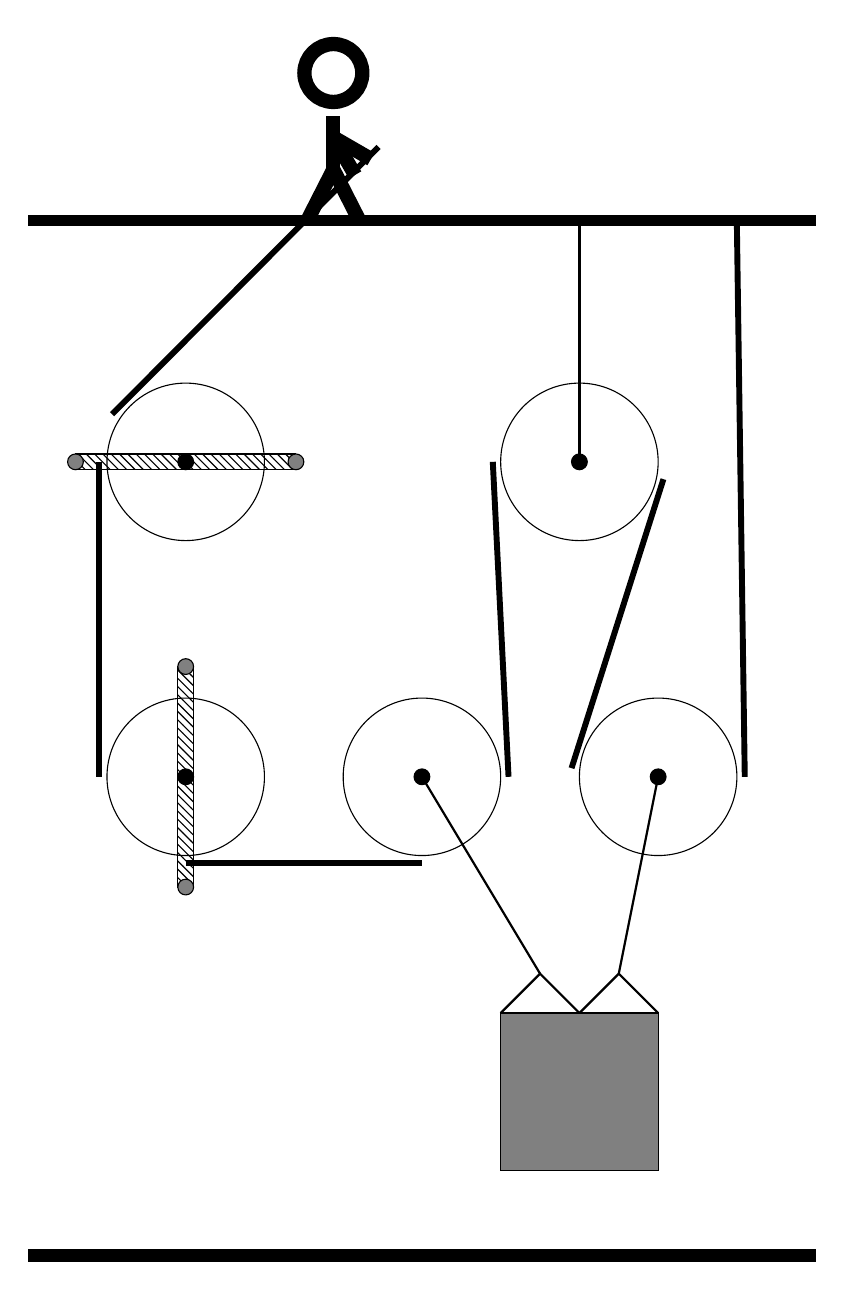
\begin{tikzpicture}
		%%%%% START %%%%%
		\draw[fill=black] (-4, 10) rectangle (6, 10.125);
		
		\draw (1, 3.0) circle (1);
		\draw[fill=black] (1, 3.0) circle (0.1);
		
		\draw (3, 7.0) circle (1);
		\draw[fill=black] (3, 7.0) circle (0.1);
		\draw[thick] (3, 7.0) -- (3, 10);
		
		\draw (4, 3.0) circle (1);
		\draw[fill=black] (4, 3.0) circle (0.1);
		
		\draw[thick] (4, 3.0) -- (3.5, 0.5);
		\draw[thick] (1, 3.0) -- (2.5, 0.5);
		\draw[thick]  (2, 0) -- (2.5, 0.5) -- (3, 0);
		\draw[thick]  (3, 0) -- (3.5, 0.5) -- (4, 0);
		\draw[fill=black!50] (2, 0) rectangle (4, -2);
		
		\draw (-2, 3.0) circle (1);
		\draw[fill=black] (-2, 3.0) circle (0.1);
		\draw[pattern=north west lines, pattern color=black] (-2.1, 4.4) rectangle (-1.9, 1.6);
		\draw[fill=black!50] (-2, 4.4) circle (0.1);
		\draw[fill=black!50] (-2, 1.6) circle (0.1);
		
		\draw (-2, 7.0) circle (1);
		\draw[fill=black] (-2, 7.0) circle (0.1);
		\draw[pattern=north west lines, pattern color=black] (-3.4, 7.1) rectangle (-0.6, 6.9);
		\draw[fill=black!50] (-3.4, 7.0) circle (0.1);
		\draw[fill=black!50] (-0.6, 7.0) circle (0.1);
		
		\draw[line width=0.75mm] (0.45, 11) -- (-2.935, 7.605);
		\centerarc[line width=0.75mm](-2, 7.0)(135:180:1.1);
		\draw[line width=0.75mm] (-3.1, 7.0) -- (-3.1, 3.0);
		\centerarc[line width=0.75mm](-2, 3.0)(180:270:1.1);
		\draw[line width=0.75mm](-2, 1.9) -- (1, 1.9);
		\centerarc[line width=0.75mm](1, 3.0)(270:360:1.1);
		\draw[line width=0.75mm] (2.1, 3.0) -- (1.9, 7.0);
		\centerarc[line width=0.75mm](3, 7.0)(-20:180:1.1);
		\draw[line width=0.75mm](4.067, 6.78) -- (2.9, 3.11);
		\centerarc[line width=0.75mm](4, 3.0)(160:360:1.1);
		\draw[line width=0.75mm](5.1, 3.0) -- (5.0, 10);
		
		\node at (-0.07, 11.2) {\Strichmaxerl[10][120][-30]};
		
		\draw[fill=black] (-4, -3) rectangle (6, -3.15);
		%%%%% END %%%%%
	\end{tikzpicture}
\end{document}